\section{Implementation Details for Viscoelasticity}\label{app:kv2d_details}

This appendix provides additional information on the numerical results for learning viscoelasticity.

\subsection{Numerical Solutions of the Unit Cell Problem}\label{app:kv2d_cell_solver}
The cell problem is discretized using a $128\times128$ uniform triangular mesh with $\bP_1$ finite elements and periodic boundary conditions. The homogenization solver uses a mixed formulation for the displacement corrector together with a Lagrange multiplier enforcing a zero-mean constraint. We use an explicit fourth-order Runge--Kutta scheme with $1024$ time steps on {$[0,1]$}. The displacement field at each time step is obtained via a direct solver. The solver is implemented in FEniCS \cite{logg2012automated, alnaes2015fenics}.

\subsection{Trajectory Sampling}\label{app:kv2d_strain_sampling}
For each independent component $a\in\{11,22,12\}$ of the macroscopic strain, we first sample the total number of control times $N_c$ uniformly from $\{3,\dots,21\}$. Let $0=t_0<t_1<\cdots<t_{N_c-1}=1$ be the control times, with the interior points sampled uniformly in $[0,1]$ and then sorted. The strain is initialized by $\overline e_a(t_0)=0$. For each $k=1,\dots,N_c-1$, we sample an independent sign $v_{a,k}\in\{-1,1\}$ and set $
    \overline e_a(t_k)
    =
    \overline e_a(t_{k-1})
    +
    \left(e_{\mathrm{max}}v_{a,k}-\overline e_a(t_{k-1})\right)
    \sqrt{t_k-t_{k-1}},$ with $e_{\mathrm{max}}=0.2$.
The values between control times are obtained via piecewise cubic Hermite interpolating polynomials (PCHIP). This procedure is applied independently to the three strain components.

\subsection{Architecture and Training}\label{app:kv2d_training}
For both the stress and kinetic response mappings in \cref{eq:F_and_G}, each Fourier neural mapping uses GELU activation, $4$ retained Fourier modes, a width of $32$, a projection width of $64$, and three layers. The temporal grids are downsampled to 256 steps for the training. The baseline dataset contains $4096$ training, $1024$ validation, and $2048$ test samples. We use the explicit Euler method to evolve the dynamics of the internal variable. Training uses the AdamW optimizer with a batch size of $32$, an initial learning rate of $10^{-3}$, and $400$ epochs. A cosine learning-rate scheduler decreases the learning rate to $10^{-5}$ by the final epoch. We use a penalty weight of $\alpha=1$ for $n_{\xi}=1$ and $\alpha=0.1$ for $n_{\xi}\in\{5, 10, 15\}$ and $\alpha=0.01$ for $n_{\xi}\in\{20,25\}$. The architecture and training are implemented in PyTorch \cite{paszke2019pytorch}.

\subsection{Voronoi Dataset}\label{app:kv2d_voronoi_dataset}
The baseline microstructures are piecewise constant on periodic Voronoi tessellations. The number of seeds is sampled uniformly from $\{5,\dots,15\}$, and the seed locations are sampled uniformly in the unit cell. Within each Voronoi region, the elastic and viscous Poisson ratios are sampled independently from $[0.05,0.45]$. The elastic and viscous Young's moduli are sampled independently from log-uniform distributions, with baseline ranges $[0.5,2.0]$ and $[0.02,0.2]$, respectively.

\subsection{Datasets with Varied Modulus Ranges}\label{app:kv2d_modulus_ranges}
For each material contrast shown in the middle panel of \cref{fig:ve_complexity}, we first generate a separate Voronoi dataset. To vary the elastic contrast range, we either set the elastic modulus to $1$ or sample it from the ranges $[0.71,1.41]$, $[0.35,2.83]$, or $[0.25,4]$. Note that even when the elastic modulus is constant, the elastic tensor remains heterogeneous because the Poisson ratio varies across each Voronoi region. To vary the viscous modulus range, we sample the viscous modulus from $[0.04,0.1]$, $[0.028,0.14]$, $[0.014,0.28]$, or $[0.01,0.4]$. Since the same Poisson ratio range is used throughout and the plane-stress isotropic tensor satisfies $\|\bA(E,\nu)\|_{{\rm op}}=E/(1-\nu)$, the material contrast in this numerical study is the ratio between the maximum and minimum values of this operator norm.

\subsection{Fitting a Linear Model}\label{app:kv2d_linear_fit}
For each microstructure, we evaluate the stress and kinetic responses of the trained neural operator model on the sampled trajectories and fit them by affine functions of the strain, strain rate, and internal state. After subtracting the fitted offsets, the linear part has the form
\begin{align*}
    \mathsf{vec}_2(\overline{\sigma}_{\rm NO})
    =A_{\dot e}\mathsf{vec}_2(\dot{\overline e})+A_e\mathsf{vec}_2(\overline e)+B\xi,\qquad\dot\xi=C\mathsf{vec}_2(\dot{\overline e})+D\xi,
\end{align*}
where $\xi\in\bR^{n_\xi}$ is the internal variable of the trained neural operator model. The tensorial form in \cref{eqns:learned_fitted_dynamics} follows from a change of coordinates. For $n_\xi=nd_{\cV^2}$ with $n\in\bN$, introduce tensors $q_{\rm NO}^{(i)}\in\cV^2$, $i=1,\dots,n$, and seek an invertible matrix $S$ such that
\begin{equation*}
    \xi=S\mathsf{vec}_2^{(n)}(q_{\rm NO}^{(1)},\dots,q_{\rm NO}^{(n)}),\qquad BS=[I\;\cdots\;I],
\end{equation*}
where each identity block has size $d_{\cV^2}\times d_{\cV^2}$. If $B$ has full row rank, such an $S$ exists, and the internal-variable contribution to the stress is $\sum_i q_{\rm NO}^{(i)}$. The matrices $A_{\dot e}$ and $A_e$ are the Mandel representations of $\bV^{\rm hom}_{\rm NO}$ and $\bE^{\rm hom}_{\rm NO}$. Partitioning $S^{-1}DS$ and $S^{-1}C$ into $d_{\cV^2}\times d_{\cV^2}$ blocks gives the Mandel representations of $\bL_{\rm NO}^{(ij)}$ and $\bK_{\rm NO}^{(i)}$, respectively. For $n_\xi=15$ in two dimensions, $d_{\cV^2}=3$ and hence $n=5$. Since $S^{-1}DS$ is similar to $D$, the eigenvalues plotted in \cref{fig:kv2d_iv_diagnostics} are invariants of the fitted linear dynamics.


\subsection{Particulate Dataset}\label{app:kv2d_particulate_dataset}

The particulate dataset consists of two-phase periodic microstructures with circular inclusions. In each sample, the elastic and viscous modulus and Poisson-ratio fields share the same inclusion geometry. The number of inclusions is drawn uniformly from $\{1,\dots,20\}$, and their sizes are chosen to give a particle area fraction in $[0.03,0.40]$ subject to non-overlap in the periodic cell. The material fields are constant on each phase. We sample elastic moduli log-uniformly from $[0.5,1.0]$ in the matrix and from $[1.0,2.0]$ in the inclusions. Viscous moduli use the reverse ordering on the logarithmic scale over $[0.02,0.2]$, so that the matrix phase is more viscous. We sample elastic and viscous Poisson ratios independently from $[0.05,0.45]$ in both phases.

\subsection{Median-Error Prediction Visualization}\label{app:kv2d_median_examples}
\Cref{fig:kv2d_prediction_median,fig:kv2d_particulate_median} show test samples whose relative stress errors are closest to the median for the baseline Voronoi and particulate datasets, respectively, using the trained neural operator model with $n_{\xi}=25$. These examples display the four scalar material fields, the imposed strain path, the predicted and reference stress components, and the predicted internal-variable trajectory. The memoryless response indicates the part of the response not captured without internal variables.

\begin{figure}[htp]
    \centering
\addtolength{\tabcolsep}{-5 pt}
    {\bf The median-error test sample: Voronoi dataset}\\
    
    \scalebox{0.85}{
    \begin{tabular}{>{\centering\arraybackslash} m{0.05\linewidth} >{\centering\arraybackslash} m{0.15\linewidth} >{\centering\arraybackslash} m{0.15\linewidth}}
       & Elasticity & Viscosity  \\
       \raisebox{5pt}{\rotatebox[origin=c]{90}{Modulus}}& 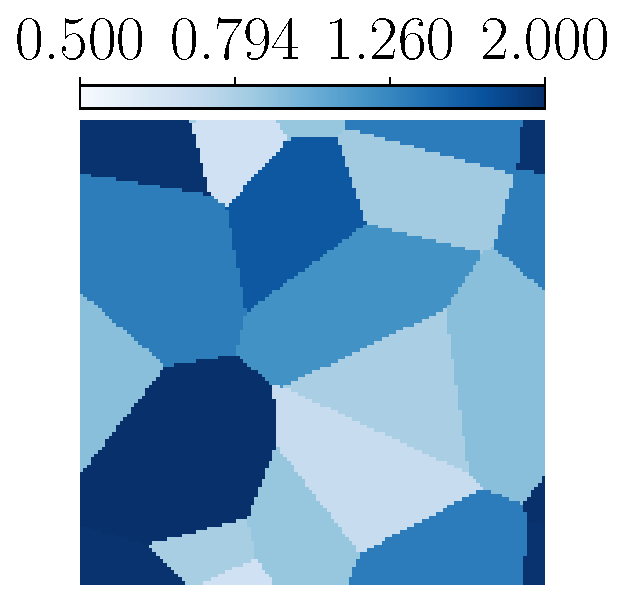
\includegraphics[width=\linewidth]{figures/elastic_modulus_iv25_median_error.pdf}  & 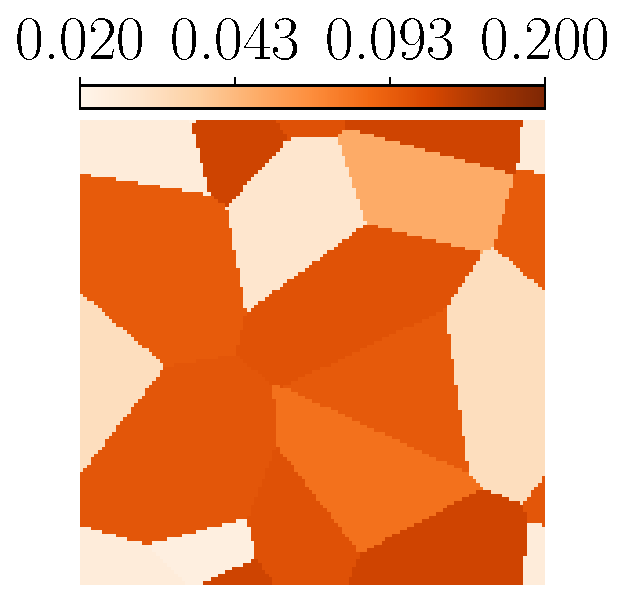
\includegraphics[width=\linewidth]{figures/viscous_modulus_iv25_median_error.pdf} \\
       \raisebox{5pt}{\rotatebox[origin=c]{90}{\makecell{Poisson\\ratio}}}& 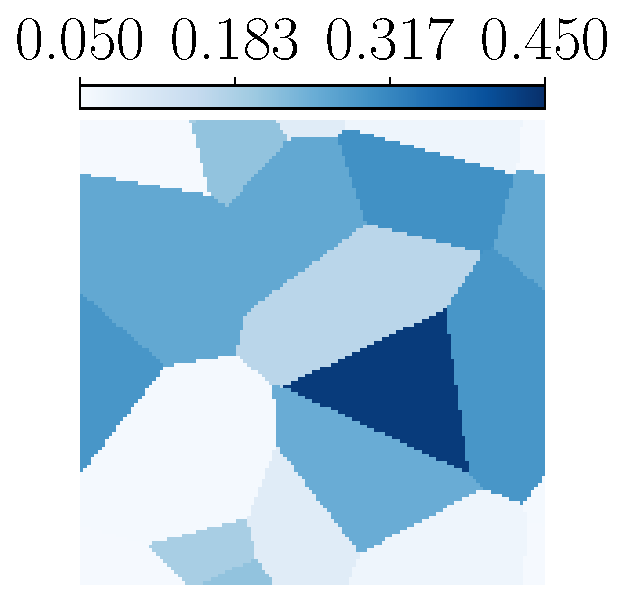
\includegraphics[width=\linewidth]{figures/elastic_poisson_iv25_median_error.pdf} & 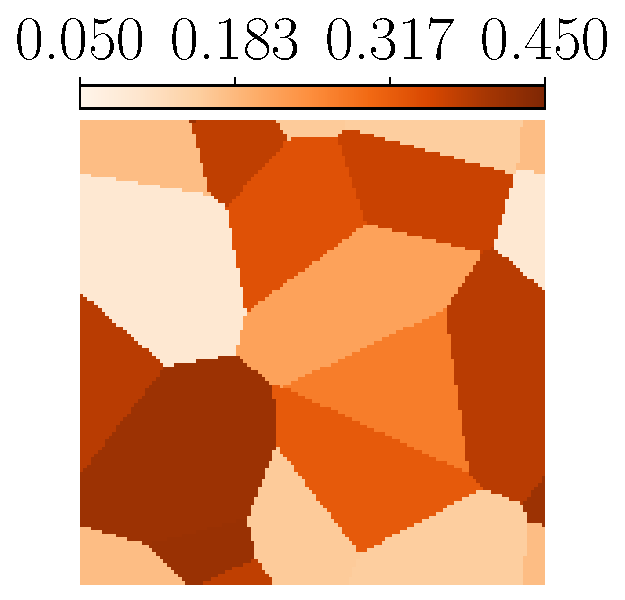
\includegraphics[width=\linewidth]{figures/viscous_poisson_iv25_median_error.pdf}
    \end{tabular}
    }
    \begin{tabular}{c c}
        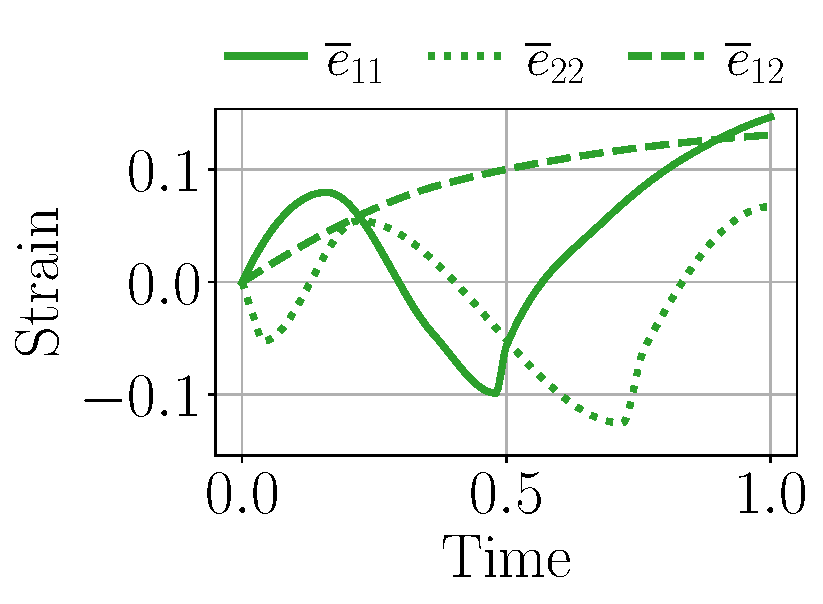
\includegraphics[width=0.245\linewidth, trim={0 0.9in 0 0},clip]{figures/strain_iv25_median_error.pdf} & 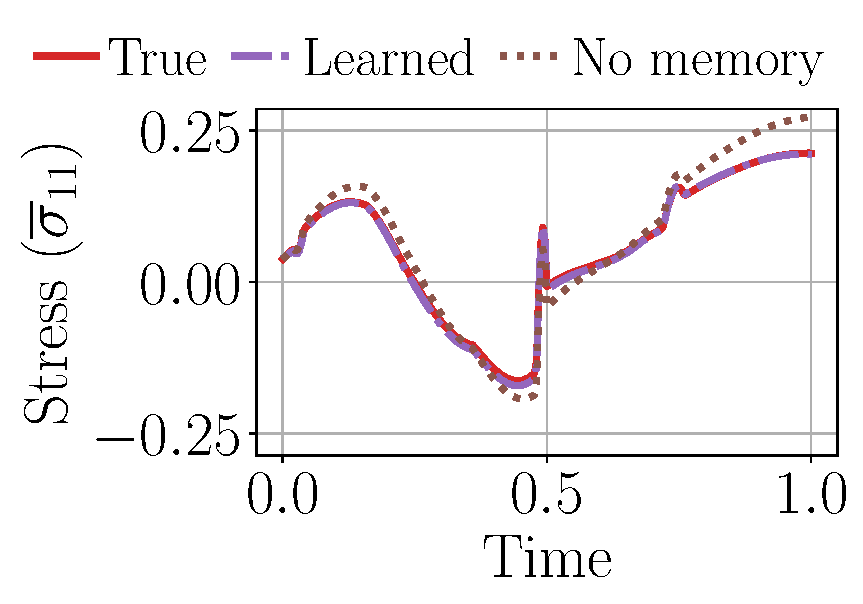
\includegraphics[width=0.25\linewidth, trim={0 0.9in 0 0},clip]{figures/stress_11_iv25_median_error.pdf}  \\
        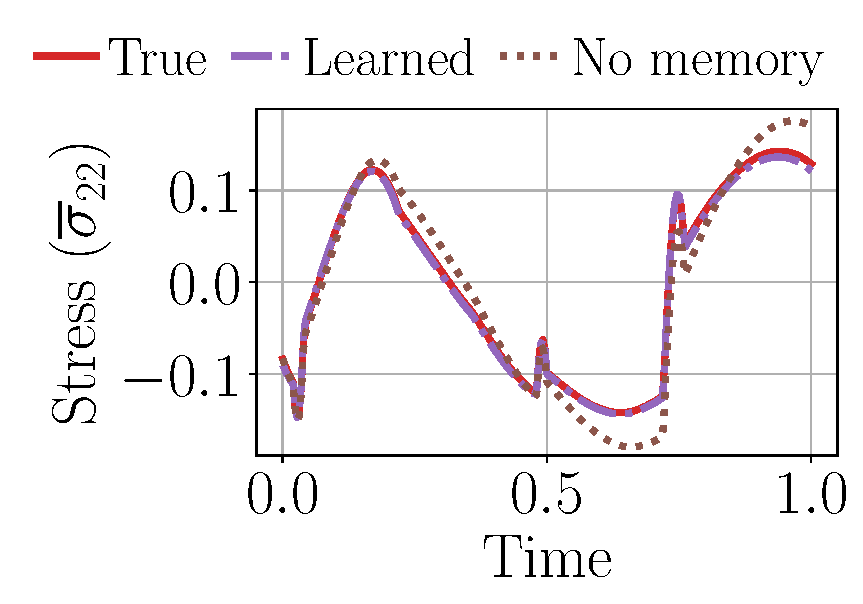
\includegraphics[width=0.25\linewidth, trim={0 0 0 0.6in},clip]{figures/stress_22_iv25_median_error.pdf} & 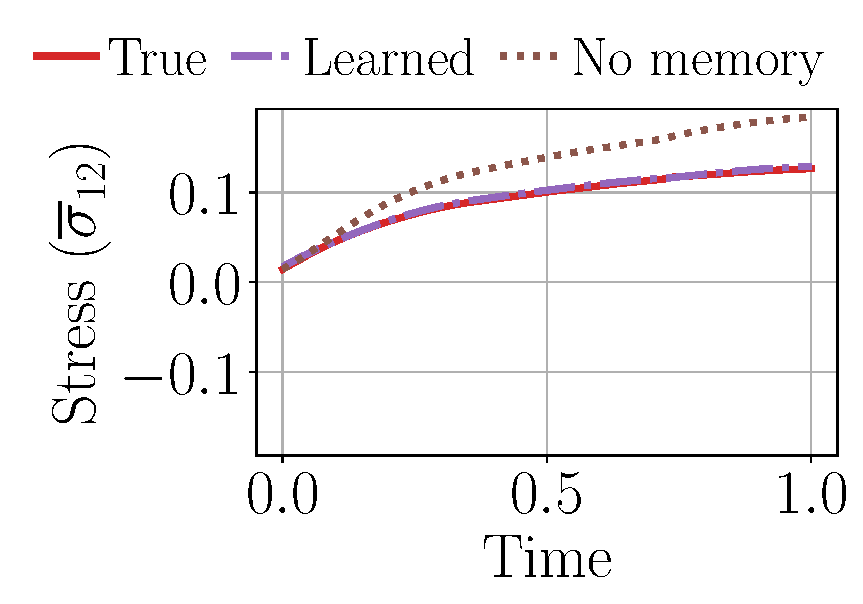
\includegraphics[width=0.25\linewidth, trim={0 0 0 0.6in},clip]{figures/stress_12_iv25_median_error.pdf}\\
        \multicolumn{2}{c}{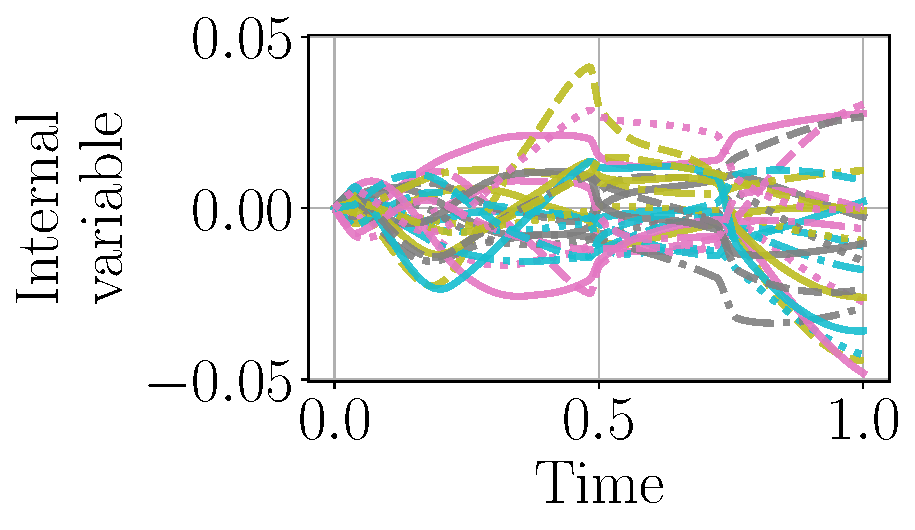
\includegraphics[width=0.27\linewidth]{figures/internal_iv25_median_error.pdf}}
    \end{tabular}\\
\addtolength{\tabcolsep}{5 pt}
    \caption{Prediction by the trained neural operator model for a viscoelasticity sample with median relative stress error, using internal-variable dimension $n_{\xi}=25$. The left panels show the microstructural property fields, while the right panels show the prescribed strain trajectory, the predicted and reference stress trajectory, and the predicted internal-variable trajectory. The memoryless prediction ($\bK=0$) is included for comparison.}
    \label{fig:kv2d_prediction_median}
\end{figure}

\begin{figure}[htp]
    \centering
\addtolength{\tabcolsep}{-5 pt}
    {\bf The median-error test sample: Particulate dataset}\\
    
    \scalebox{0.85}{
    \begin{tabular}{>{\centering\arraybackslash} m{0.05\linewidth} >{\centering\arraybackslash} m{0.15\linewidth} >{\centering\arraybackslash} m{0.15\linewidth}}
       & Elasticity & Viscosity  \\
       \raisebox{5pt}{\rotatebox[origin=c]{90}{Modulus}}& 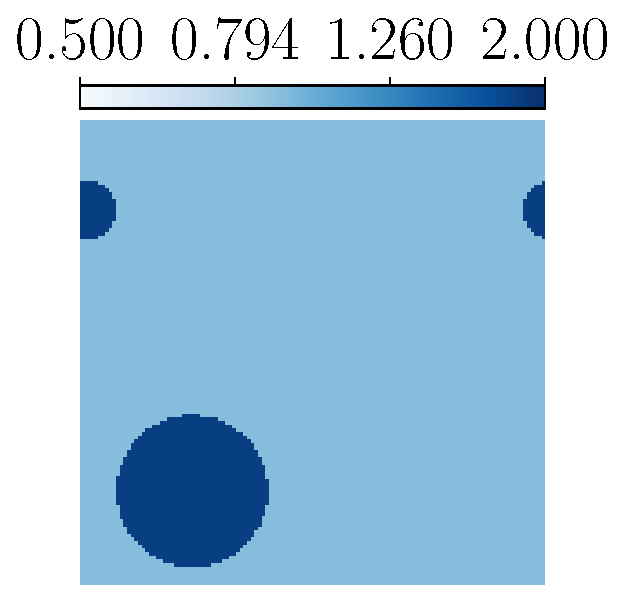
\includegraphics[width=\linewidth]{figures/elastic_modulus_particulate.pdf}  & 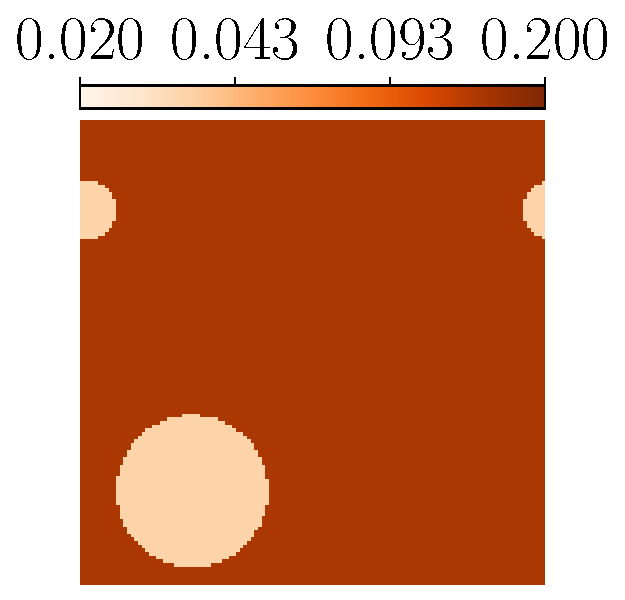
\includegraphics[width=\linewidth]{figures/viscous_modulus_particulate.pdf} \\
       \raisebox{5pt}{\rotatebox[origin=c]{90}{\makecell{Poisson\\ratio}}}& 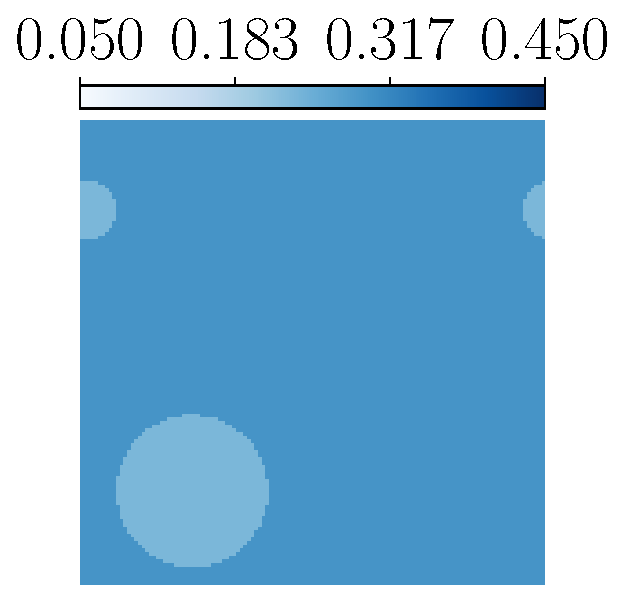
\includegraphics[width=\linewidth]{figures/elastic_poisson_particulate.pdf} & 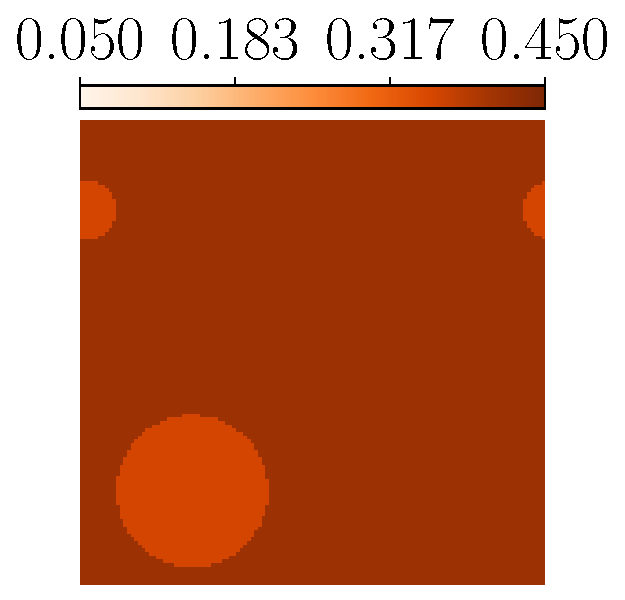
\includegraphics[width=\linewidth]{figures/viscous_poisson_particulate.pdf}
    \end{tabular}
    }
    \begin{tabular}{c c}
        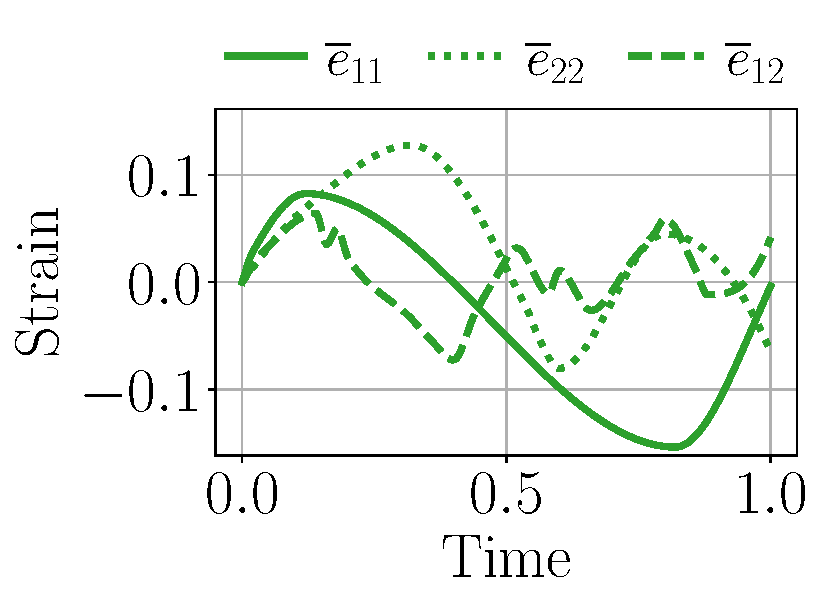
\includegraphics[width=0.245\linewidth, trim={0 0.9in 0 0},clip]{figures/strain_particulate.pdf} & 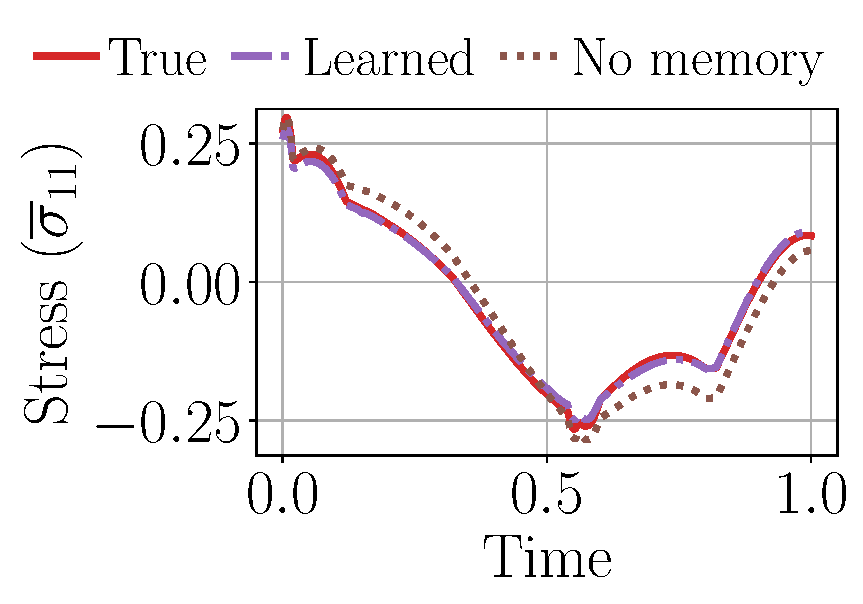
\includegraphics[width=0.25\linewidth, trim={0 0.9in 0 0},clip]{figures/stress_11_particulate.pdf}  \\
        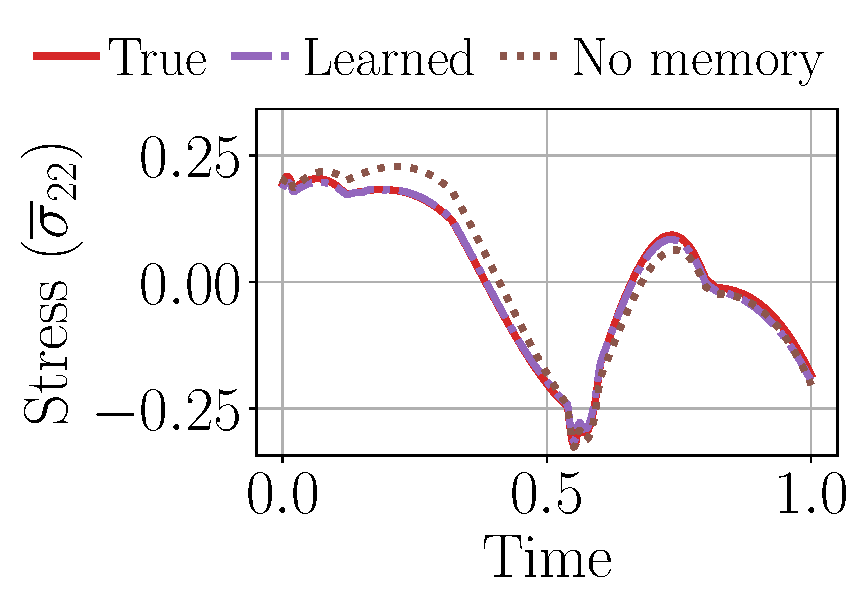
\includegraphics[width=0.25\linewidth, trim={0 0 0 0.6in},clip]{figures/stress_22_particulate.pdf} & 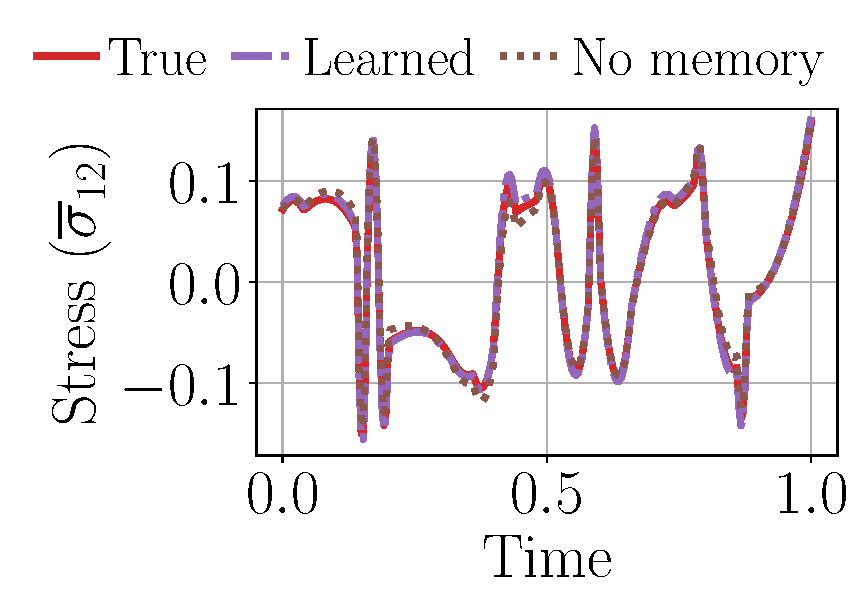
\includegraphics[width=0.25\linewidth, trim={0 0 0 0.6in},clip]{figures/stress_12_particulate.pdf}\\
        \multicolumn{2}{c}{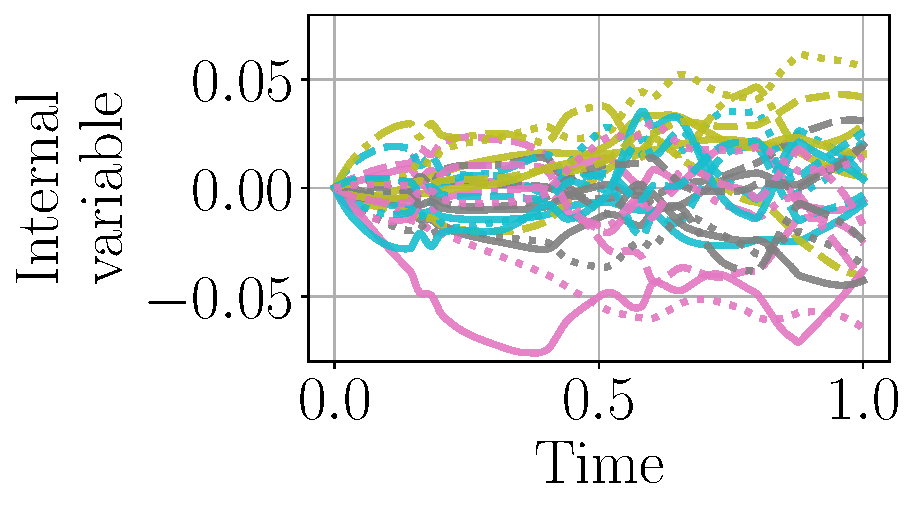
\includegraphics[width=0.27\linewidth]{figures/internal_particulate.pdf}}
    \end{tabular}\\
\addtolength{\tabcolsep}{5 pt}
    \caption{Prediction by the trained neural operator model for a particulate viscoelasticity sample with median relative stress error, using internal-variable dimension $n_{\xi}=25$. The left panels show the microstructural property fields, while the right panels show the prescribed strain trajectory, the predicted and reference stress trajectory, and the predicted internal-variable trajectory. The memoryless prediction ($\bK=0$) is included for comparison.}
    \label{fig:kv2d_particulate_median}
\end{figure}
